\chapter{Introduction to Organisation}\hrule
\label{Chapter:1}
% =====================================================================================================
\section {Organisation Profile and History}

I had my Six Weeks Training at Naresh Teachnology, Hydrabad. Naresh Technologies was founded in Nov, 2004 by Mr. Naresh and some of its colleagues. It is an ISO 9001-2008 certified company.
\\
\section {Mission And Vision}


To enrich the knowledge & skill sets of young software engineers by providing value added training in the areas of Software Development & Testing.

To serve the industries by providing trained human resources in the above areas.

To provide quality Software Training & Consulting Services in the areas of J2EE, .NET, ERP, Database Administration, Testing, Content Management with Live Projects.
\\
\section {Management Team}
NareshIT Management have more than 15 years of experience in IT Industry in various domains.  With a motto of empowering youth in IT education to IT Careers, Management has shown great interest in this field and was able to see vision of the company goal.  Strategies adopted to make the students ready for the Job are different and hence able to see the positive response from Job seekers and hiring companies.  Developing the core team members and encouraging software trainers to deliver World Class Software Training keeping the standards in mind which is our passion and quickly adopting to latest technology trends and cutting-edge technologies..
\\
\\
NareshIT has associated with National and International organizations for maintaining and developing the Standard & Quality gives an edge to be with IT Industry heights.  The leadership quality of the management drives the employees to be satisfactory level and to execute the strategies with high Quality.
\\
\\
Two words that perfectly encapsulate their commitment to service: whatever they do, they do it precisely and they do it right. They use new ideas, technology and expertise for development of products, services, systems and people and make them more competitive. Their Training Services are based on latest technologies which inspire their customers. Team NareshIT create optimal software solutions and guarantee high-quality customer support.
\\
\\
The institute has more than 50K students who are trained in various latest software technologies in a year. The company has excellent history in software training and the company is also keenly looking forward to continue its legacy.

\chapter{Introduction to Project}\hrule
\label{Chapter:2}
% =====================================================================================================
\section{Overview}

This project sequentially applies a set of Hadoop techniques to gain insights from the Direct Marketing campaign of a Portuguese Banking Institution.Hadoop Environoment analysis of this data will benefit the business processes of the Banking and Financial Management Industry. \\
\\
The Portuguese Bank that initiated the telemarketing campaign, (that provided the data examined by this project), contacted potential savings account depositors for a 5 year period, 2008 through 2013. This data therefore reflects the influence of the financial crisis of 2008. The original study gathered information on 150 different data categories, that covered information about clients, the bank’s products, social factors and economics. The original data was processed through data modelling with the objective of reducing the feature set. The data examined during that process was pre-July 2012 data. The result of the feature selection was a dataset of 22 of the starting 150 categories. This document examines the dataset of 22 marketing campaign metadata categories. A final set of 2 data categories, “Housing” and “Loan”, was determined as having the greatest effect on bank customers subscribing to “Term Deposit” accounts. Thereby, allowing for prediction of Term Deposit subscriptions by bank customers.\\
\\
In 1963, the Supreme Court held that the antitrust laws, and in particular section 7 of the Clayton Act (1914), applied to banking. In 1966, Congress reaffirmed the Supreme Court’s opinion regarding application of the Clayton Act via amending the Bank Merger Act of 1960, and the Bank Holding Company Act of 1956. In 1978, Congress further reaffirmed the Supreme Court’s opinion via passing the Change in Bank Control Act.
\\
Modern geographic and product definitions used by banking institutions were examined by the Supreme Court during the Philadelphia National Bank case. The Court determined that because banking institutions were mostly local in scope, the local geographic area is relevant for analysis of competition in banking. The Supreme Court determined that “the cluster of products (various kinds of credit) and services (such as checking accounts and trust administration) denoted by the term ‘commercial banking’ composes a distinct line of commerce.” Therefore, local banking services and products are possibly free of effective competition from other banking institutions because of the locally distinctive characteristics of the services. Local banking institutions are also possibly exempted from competition by cost advantages, and customer preferences. Substitution of these services was often not possible on a local level.\\
\\
Since 1963, antitrust courts have had to adapt to financial sector changes involving product line diversity, and access to local markets by national institutions. However, not until recently has evidence emerged of a shift to banking with services and products provided by national institutions. Antitrust Courts now have the statistical evidence needed for a redefinition of banking services and products. The evidence of changes in financial services includes research on the Survey of Consumer Finances (SCF) and the Surveys of Small Business Finances (SSBF) in 1993, 1998, and 2003.
\\
\\
The SSBF indicated that within the USA, small businesses obtain an average of two financial services from a local financial institution, and a local depository institution, that are primarily commercial banks. This is contrasted by small businesses obtaining only one banking service from a non-local institution. From 1989 to 1998, evidence of a shift to non-local services by individual households began to appear. During that time, consumers had began to rely on an increased amount of financial services, and the percentage of financial services obtained from one institution had decreased. As of 2003, most banking services and products were obtained by households and businesses from local banking institutions.
\\
\\
In 1998, 82 percent of all small business financial services were obtained from local banking institutions, with 94 percent of checking and savings services, and over 75 percent of financial management services. A survey conducted by the National Federation of Independent Businesses found that small businesses perceived local banking as a preferential option. Past SCF research indicated that households primarily relied on local banking institutions for banking transactions, certificates of deposits, and lines of credits. Yet households had started to rely on non-local services for alternate forms of banking. Even though the local areas in question had divergent deposit and loan rates, the suppliers of banking services remained local. In the early 1990s, higher loan interest rates, and significantly lower deposit interest rates were available via local banking.
\\
\\
The period from 2008 - 2013 represented an accelerated period of expansion of non-local, internet based banking options for individuals searching for banking services. During that period of time the services from local banks that were sought out by customers moved to national institutions. In order for new large national banking enterprises to sell banking products to previously local banking customers, an understanding of local factors of banking product selection is required. In 1994, only 1 percent of banking institutions did not have a branch in the local marketing area their customers lived in. By 2004, 18 percent of banking institutions did not have a local branch in order to respond to the individual needs of their customers.
\\
\\
Via Customer Segmentation with Data Science techniques, the previous local demands of banking services are conformable to corresponding segments of the population, determined by Customer Data characteristics. This segmentation is then usable by banking regulation institutions, and by businesses seeking to provide innovative banking services on a national scale. The effects of national banking services on all populations, national and local, are measureable with the causes of interest by individuals defined by data categories that are measurable with a national or local focus.
\\
\\
The Financial Services Modernization Act of 1999, has introduced complexity to the definition of banking service demand, and therefore the measurement of banking service marketing effectiveness and scope. As a result, the variety of banking services has grown to encompass the growing complexity of services defined as banking services.
\\
\\
Via the internet, banking service providers have expanded the range of services they have traditionally offered to customers. The expanded services now exist has separate business areas that provide deposit, loan, mortgage, credit, transaction card, vehicle loan, and business loan services. High risk short term loans, and investment brokerages, have become available with the same convenience of all other types of banking services. The origin corporations associated with new internet banking products have been obscured. Thereby, acceptance of banking product services has become independent of the enterprise providing the service.
\\
\\
Thereby, a customer-based focus of analysis of banking services via Data Science, allows for understanding of the possible effects of the concentration of a wide variety of banking resources into a small group of national enterprises. Divergent demographic and economic characteristics of consumers are now examinable independent of geographic area, in order to determine the likelihood of procurement of financial services.
\section{Why we Analysize Bank Marketing Data ?}

 Reason behind the examination of the telemarketing data of this Portuguese Bank is important is the controversy related to local marketing of banking products. National networks of large banks have encroached on the accessibility in local areas to small, locally-based banks. This expansion into the local territories of small banks has increased with legislation friendly to powerful, national banking enterprises. The results of this phenomena are the movement of bank deposit funds to large national banks, and the setting of prices for banking services on a non-local scale, the ubiquitousness of compatible ATM machines, and the availability of internet banking.
 \\
 \\
 Thereby, not only is the availability of local banks affected by the expansion of national banks, the availability of banking products unique to local banks are also affected. Competition between banking institutions have moved from a local focus defined as the area of one city or one county, to a national focus defined as the area of one country. The large national banks in question are not limited to supplying banking products and services only, unlike previous local banks. The Horizontal Merger Guidelines of the Department of Justice and Federal Trade Commission, defines a market as a “product or group of products and a geographic area such that a hypothetical profit-maximizing firm, not subject to price regulation, that was the only present and future producer or seller of those products in that area likely would impose at least a ‘small but significant and nontransitory’ increase in price, assuming the terms of sale of all other products are held constant.”
 \section {Exitsing System}
 
 As day by day, the data used increases and therefore a better way of handling such a huge amount of data is becoming a hectic task. The traditional approach of data storage and analysis is RDBMS.RDBMS is mainly for structured data only.It stores the average size of data(Gbs).For RDBMS we take license so cost is high.
 \\
 \\
  When a size of data is too big for complex processing and storing or not easy to define the relationships between the data, then it becomes difficult to save the extracted information in an RDBMS with a coherent relationship.
  \\
  \\
  By the above comparison, we have come to know that HADOOP is the best technique for handling Big Data compared to that of RDBMS.
  
  
\section{Working Directory And Required Packages}
 
 The  is used for interactive programming of the Hadoop analysis, of the Bank Marketing data. In addition to the basic capabilities of the HDFS , Pig,Hive,HBase,Sqoop,Hcatlog  are used for the analysis. The Bank Marketing datasets are cleaned via use of “strings as factors” importing of the unorganized .csv files containing the data. The cleaned datasets are then stored as new .csv files, with new names designating that they are the cleaned version of the original dataset files.
 
 Dataset link: https://archive.ics.uci.edu/ml/datasets/bank+marketing\\
 Go to data folder and then “bank.zip”
\subsection{Functional Requirements}
\begin{itemize}
	\item Setup of Hadoop Environment.
	\item PC needs to have atleast 8 GB Ram and atleast 100GB  of external usable memory.
	\item PC should have Ubuntu 16.4v or Windows 7 or above.
\end{itemize}
\section{Feasibility Study}
A feasibility study is used to determine the viability of an idea, such as ensuring a project is legally and technically feasible as well as economically justifiable. It tells us whether a project is worth the investment—in some cases, a project may not be doable. There can be many reasons for this, including requiring too many resources, which not only prevents those resources from performing other tasks but also may cost more than an organization would earn back by taking on a project that isn’t profitable.\\
\\
The application is fully feasible. It just needs a working internet connection,PC have atleast 8 GB RAM above. It is fully feasible if it is also deployed on a large scale.\\
The Project can also be upgraded further and can be deployed on large scale depending upon the need of business plan.\\
\begin{enumerate}
	\item \textbf{Technical Feasibility :} The Project is fully feasible on technical terms. I have PC and required 8 GB Ram for development purpose.\\
	I will use cloudera Environment to deploy backend as it is frees.\\
	The version control system is completely free and the website Github.com is also free for Open Source Projects.
   \item \textbf{Economic Feasibility :} The Project is fully economically feasible as it has free and open source tools being used while developing the system.\\
   The Tableau technology is free for 14 days but for student it is free for one years.
   \item \textbf{Legal Feasibility :} The Project doesn't violates any legal rights and will credit the author of open Source Library used while developing the project.\\
   The project will be available in open source under \textbf{GPLv3} license.\\
   \\
   \textbf{What is GPLv3 License?}
   \begin{itemize}
   	\item The source code must be made public whenever a distribution of the software is made.
   	\item Modifications of the software must be released under the same license.
   	\item Changes made to the source code must be documented.
   	\item If patented material was used in the creation of the Project, it grants the right for users to use it. If the user sues anyone over the use of the patented material, they lose the right to use the Project.\\
   \end{itemize}
 
   \item \textbf{Operational Feasibility : } As the Project satisfies the functional and non functional requirements, the Project will be fully operational once it releases.
   
   \item \textbf{Scheduling Feasibility : } The project release targets for different versions are practical and have plenty of time develop and debug the Project before release.
\end{enumerate}

\section{Objectives of the Project }
The main objective of this project to how to increases bank marketing to analize of bank data sets.The objective of the classification is to predict if the client will subscribe to a Term Deposit. “Data Classification” is the use of Hadoop techniques to organize datasets into related sub-populations, not previous specified in the dataset.




\chapter{Product Design}\hrule
\label{Chapter:3}
% =====================================================================================================

\section{Product Perspective}
This Project utilizes Data Classification to examine a dataset related with direct marketing campaigns (phone calls) of a Portuguese banking institution. The objective of the classification is to predict if the client will subscribe to a Term Deposit. “Data Classification” is the use of Hadoop techniques to organize datasets into related sub-populations, not previous specified in the dataset. This can uncover hidden characteristics within data, and identify hidden categories that new data belongs within.
\section{Characteristics of the Data}
The dataset examined by this Project was collected from a telemarketing campaign by a Portuguese banking institution. Occasionally, customers were contacted more than once, in order to attempt to sell Term Deposit subscriptions. The Bank Marketing dataset includes 45211 records, with 21 observations per record. Each record includes 20 explanatory observations about the client contacted, and 1 response observation of whether the client subscribed to a Term Deposit.
\\
\\
The 20 explanatory observations contain 4 types of client data:The 20 explanatory observations contain 3 types of client data:
\begin{enumerate}
	\item Customer data: age, job, marital status, education, default, housing and loan.
	\item Telemarketing data: contact, month, day of the week, and duration.
	\item Other data: campaign, past days, previous, and past outcome.
\end{enumerate}
\section{Definition of Input Variables}
age - Age of the client- (numeric)

job - Client’s occupation - (categorical)
(admin, bluecollar, entrepreneur, housemaid, management, retired, selfemployed, services, student, technician, unemployed, unknown)

marital - Client’s marital status - (categorical)
(divorced, married, single, unknown, note: divorced means divorced or widowed)

education - Client’s education level - (categorical)
(basic.4y, basic.6y, basic.9y, high.school, illiterate, professional.course, university.degree, unknown)

default - Indicates if the client has credit in default - (categorical)
(no, yes, unknown)

housing - Does the client as a housing loan? - (categorical)
(no, yes, unknown)

loan - Does the client as a personal loan? - (categorical)
(no, yes, unknown’)

contact - Type of communication contact - (categorical)
(cellular, telephone)

month - Month of last contact with client - (categorical)
(January - December)

day_of_week - Day of last contact with client - (categorical)
(Monday - Friday)

duration - Duration of last contact with client, in seconds - (numeric)
For benchmark purposes only, and not reliable for predictive modeling

campaign - Number of client contacts during this campaign - (numeric)
(includes last contact)

pdays - Number of days from last contacted from a previous campaign - (numeric)
(999 means client was not previously contacted)

previous - Number of client contacts performed before this campaign - (numeric)

poutcome - Previous marketing campaign outcome - (categorical)
(failure, nonexistent , success)

emp.var.rate - Quarterly employment variation rate - (numeric)

cons.price.idx - Monthly consumer price index - (numeric)

cons.conf.idx - Monthly consumer confidence index - (numeric)

euribor3m - Daily euribor 3 month rate - (numeric)

nr.employed - Quarterly number of employees - (numeric)

Output variable (desired target) - Term Deposit - subscription verified
(binary: ‘yes’,‘no’)
\section{Sample of Records}
\begin{figure}[h!]
	\centering
	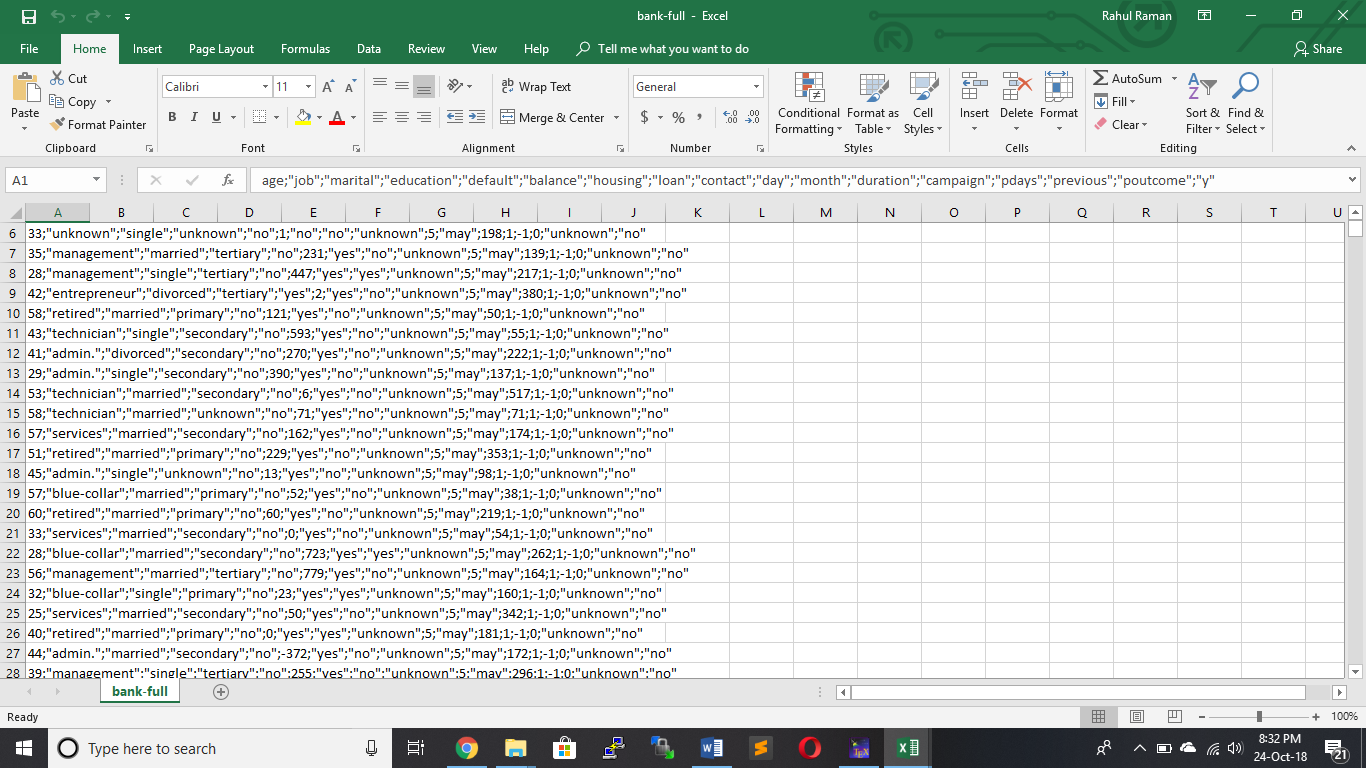
\includegraphics[width=0.75\linewidth]{sample_of_Data.png}
	\caption{Sample of DataSets}
	\label{fig:flowchart}
\end{figure}

\section{Flow Chart}
The Flow of Data Classification is looks like-
\begin{figure}[h!]
	\centering
	\includegraphics[width=0.75\linewidth]{flow_chart.png}
	\caption{Data Classification Flow chart}
	\label{fig:flowchart}
\end{figure}

\section{Assumptions and Dependencies}
\begin{itemize}
	\item Company is assumed to be using PC having  atleast 8 GB RAM.
	\item Company is assumed to have working internet connection.
	\item The Bank Marketing dataset contains numeric variables, (useful for predictive analytics and machine learning), categorical variables, discrete and continuous variables. 19 of the 20 explanatory variables initially appear useful for prediction of future Term Deposit subscriptions.
	\item The explanatory variable, “duration”, records the amount of time the telemarketer spends speaking with customers, and therefore isn’t a factor in real-time prediction of likelihood of obtaining a Term Deposit. \\
	\\
\end{itemize}
\section{Specific Requirements}
\begin{itemize}
	\item PC have ubuntu 16.4,windows 7.0 or above os.
	\item Working internet connection.
	\item Minimum 8 GB Ram and 100 GB external memory.
\end{itemize}
\chapter{Development and Implementation}\hrule
\label{Chapter:4}
% =====================================================================================================
\section{Data Importing}

In order to begin processing the Bank Marketing Datasets, “bank.csv”  are imported into the Hadoop environment and stored in HDFS Location. After import of the data, we find the datasets contains 41188 records of 21 different observations/variables.
\subsection{Hadoop File Distribution System(HDFS) }
Hadoop File System was developed using distributed file system design. It is run on commodity hardware. Unlike other distributed systems, HDFS is highly faulttolerant and designed using low-cost hardware.

HDFS holds very large amount of data and provides easier access. To store such huge data, the files are stored across multiple machines. These files are stored in redundant fashion to rescue the system from possible data losses in case of failure. HDFS also makes applications available to parallel processing.
\subsection{Features of HDFS}
\begin{itemize}
\item It is suitable for the distributed storage and processing.
\item Hadoop provides a command interface to interact with HDFS.
\item The built-in servers of namenode and datanode help users to easily check the status of cluster.
\item Streaming access to file system data.
HDFS provides file permissions and authentication.
\subsection{Architecture of HDFS}
The following fig shows architecture of HDFS-
\begin{figure}[h!]
	\centering
	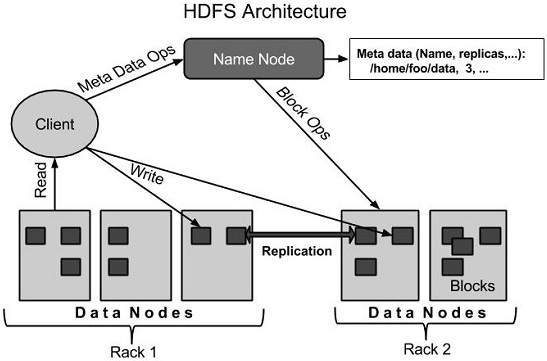
\includegraphics[width=\linewidth]{hdfs_architecture.jpg}
	\caption{Architecture of HDFS}
\end{figure}
\section{Supporting Tools}
\subsection{Pig}
Apache Pig is an abstraction over MapReduce. It is a tool/platform which is used to analyze larger sets of data representing them as data flows.we can perform all the data manipulation operations in Hadoop using Pig.
\\ 
\\
To write data analysis programs, Pig provides a high-level language known as Pig Latin. This language provides various operators using which programmers can develop their own functions for reading, writing, and processing data.
\\
\\
To analyze data using Apache Pig, programmers need to write scripts using Pig Latin language. All these scripts are internally converted to Map and Reduce tasks. Apache Pig has a component known as Pig Engine that accepts the Pig Latin scripts as input and converts those scripts into MapReduce jobs.
\subsection*{Features of Pig}

Apache Pig comes with the following features −
\begin{itemize}
\item Rich set of operators − It provides many operators to perform operations like join, sort, filer, etc.

\item Ease of programming − Pig Latin is similar to SQL and it is easy to write a Pig script if you are good at SQL.

\item Optimization opportunities − The tasks in Apache Pig optimize their execution automatically, so the programmers need to focus only on semantics of the language.

\item Extensibility − Using the existing operators, users can develop their own functions to read, process, and write data.

\item UDF’s − Pig provides the facility to create User-defined Functions in other programming languages such as Java and invoke or embed them in Pig Scripts.

\item Handles all kinds of data − Apache Pig analyzes all kinds of data, both structured as well as unstructured. It stores the results in HDFS.
\end{itemize}
\subsection{Hive}

Hive is a data warehouse infrastructure tool to process structured data in Hadoop. It resides on top of Hadoop to summarize Big Data, and makes querying and analyzing easy.
\\
\\
Initially Hive was developed by Facebook, later the Apache Software Foundation took it up and developed it further as an open source under the name Apache Hive. It is used by different companies. For example, Amazon uses it in Amazon Elastic MapReduce.
\subsection*{Hive is Not}
\begin{itemize}
	\item A relational database
	\item A design for OnLine Transaction Processing (OLTP)
	\item A language for real-time queries and row-level updates
\end{itemize}
\subsection*{Features of Hive}
\begin{itemize}
	\item It stores schema in a database and processed data into HDFS.
\item It is designed for OLAP.
\item It provides SQL type language for querying called HiveQL or HQL.
\item It is familiar, fast, scalable, and extensible.
\end{itemize}
\subsection*{Architecture of Hive}
The following fig shows architecture of Hive-
\begin{figure}[h!]
	\centering
	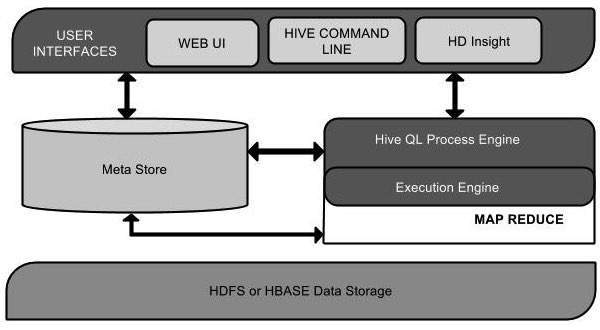
\includegraphics[width=\linewidth]{hive_architecture.jpg}
	\caption{Architecture of Hive}
\end{figure}
\subsection{SQOOP}
Sqoop is a tool designed to transfer data between Hadoop and relational database servers. It is used to import data from relational databases such as MySQL, Oracle to Hadoop HDFS, and export from Hadoop file system to relational databases.It is provided by the Apache Software Foundation.
\subsection*{How Sqoop Works?}
The following image describes the workflow of Sqoop-
\begin{figure}[h!]
	\centering
	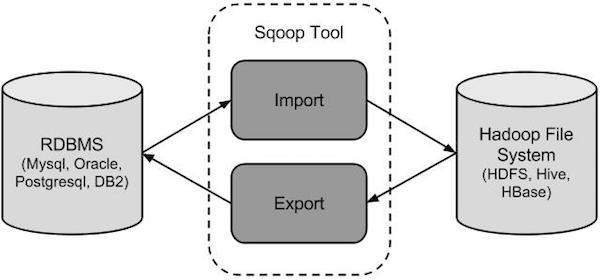
\includegraphics[width=\linewidth]{sqoop_work.jpg}
	\caption{Workflow of Sqoop}
\end{figure}
\subsection{HCatalog}
HCatalog is a table storage management tool for Hadoop. It exposes the tabular data of Hive metastore to other Hadoop applications. It enables users with different data processing tools (Pig, MapReduce) to easily write data onto a grid. It ensures that users don’t have to worry about where or in what format their data is stored.
\\
\\
HCatalog works like a key component of Hive and it enables the users to store their data in any format and any structure.
\subsection*{Architecture of HCatalog}
The following illustration shows the overall architecture of HCatalog.
\begin{figure}[h!]
\centering
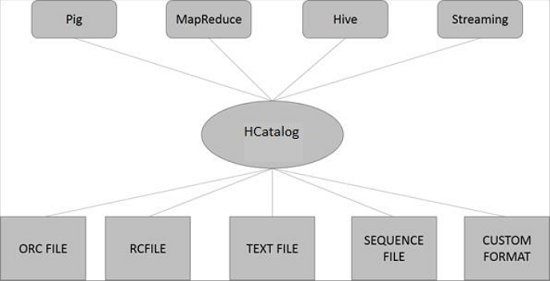
\includegraphics[width=\linewidth]{Hcatalog_architecture.jpg}
\caption{Architecture of HCatalog}
\end{figure}
\subsection{Tableau}
Tableau is a Business Intelligence tool for visually analyzing the data. Users can create and distribute an interactive and shareable dashboard, which depict the trends, variations, and density of the data in the form of graphs and charts. Tableau can connect to files, relational and Big Data sources to acquire and process data. The software allows data blending and real-time collaboration, which makes it very unique. It is used by businesses, academic researchers, and many government organizations for visual data analysis. It is also positioned as a leader Business Intelligence and Analytics Platform in Gartner Magic Quadrant.

\section{Implementation with ScreenShots}
\\
\title{Data Visualization of the Bank Dataset}
\\
%
 Bank - Maritial looks like-
\begin{figure}[h!]
	\centering
	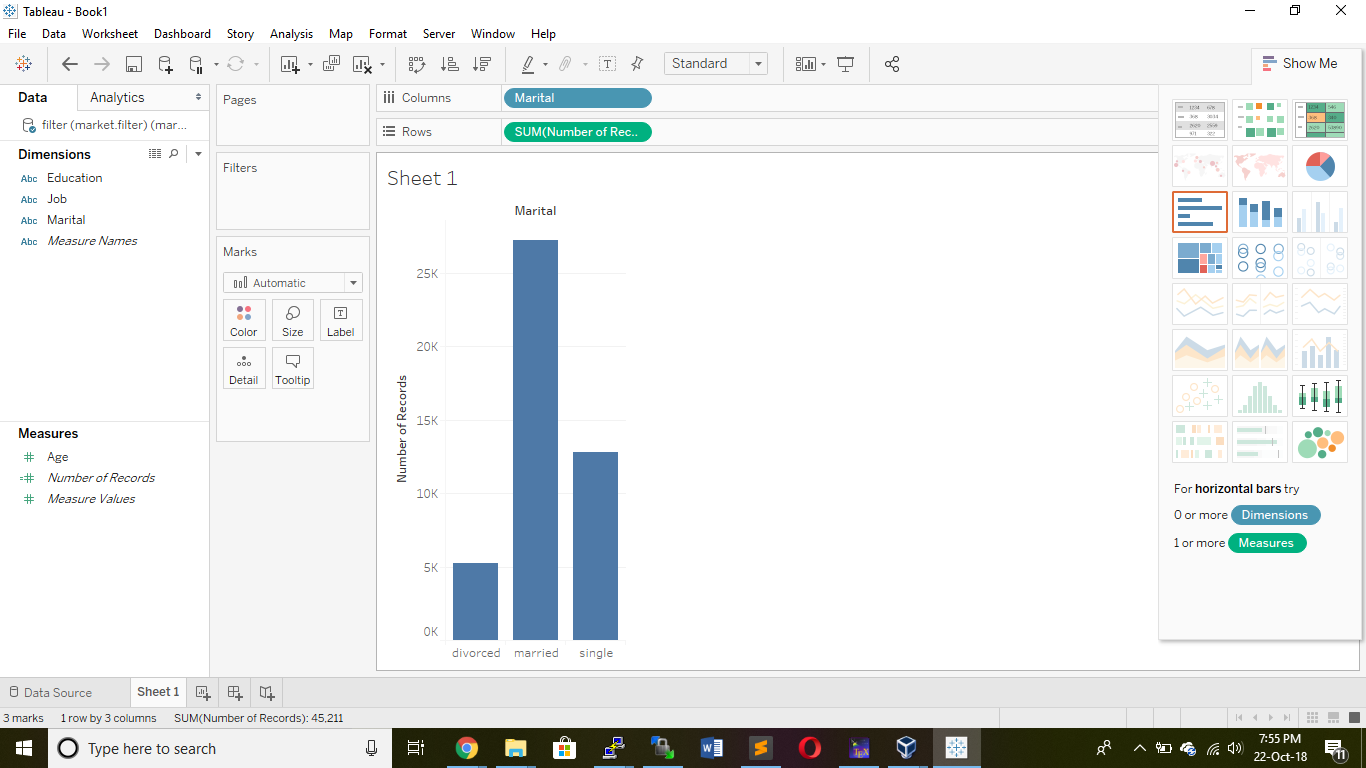
\includegraphics[width=\linewidth]{sc1.png}
	\caption{Maritial vs Count}
\end{figure}
%
%
maritial status - Married-
\begin{figure}[h!]
	\centering
	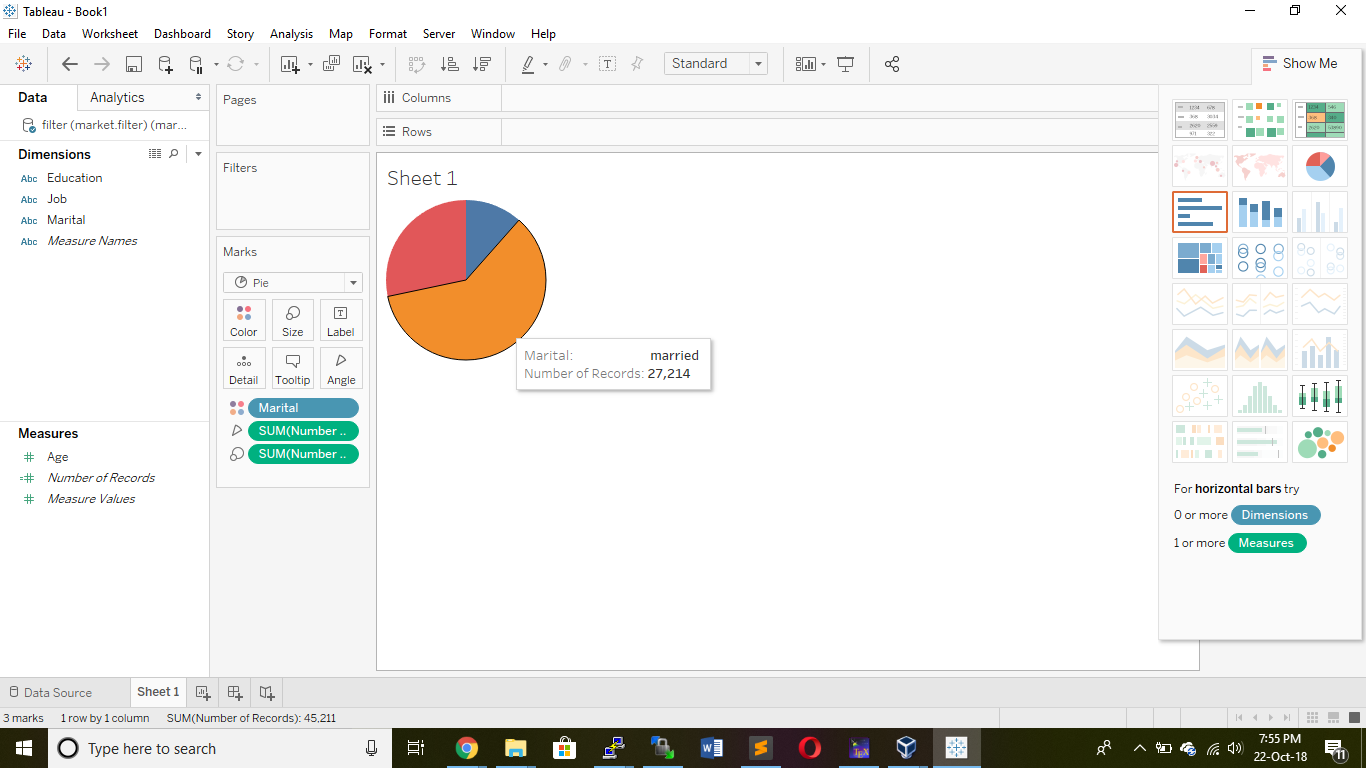
\includegraphics[width=\linewidth]{sc2.png}
	\caption{Pie chart of married vs count}
\end{figure}
%
\\
\\
maritial status - Single-
\begin{figure}[h!]
	\centering
	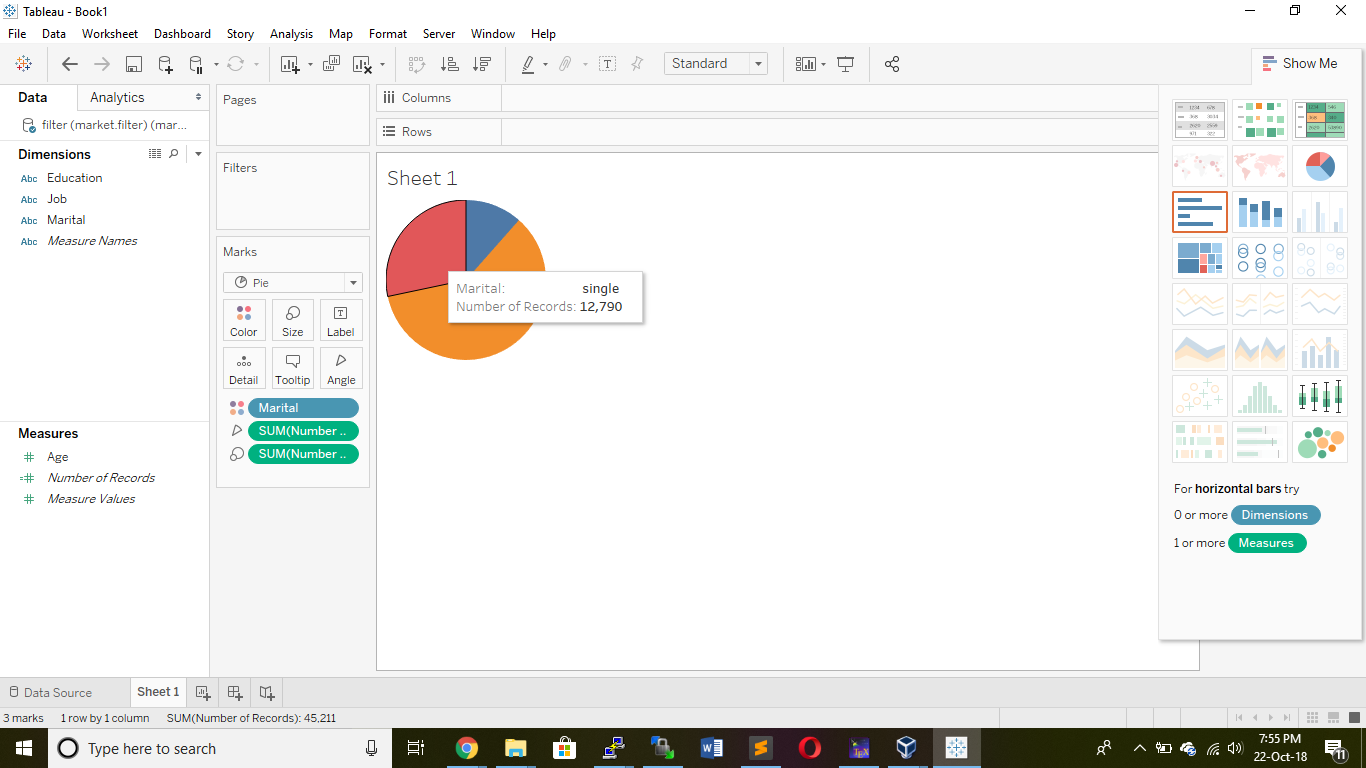
\includegraphics[width=\linewidth]{sc3.png}
	\caption{Pie chart of single vs count}
\end{figure}
\\
\\
maritial status - Divorced-
\begin{figure}[h!]
	\centering
	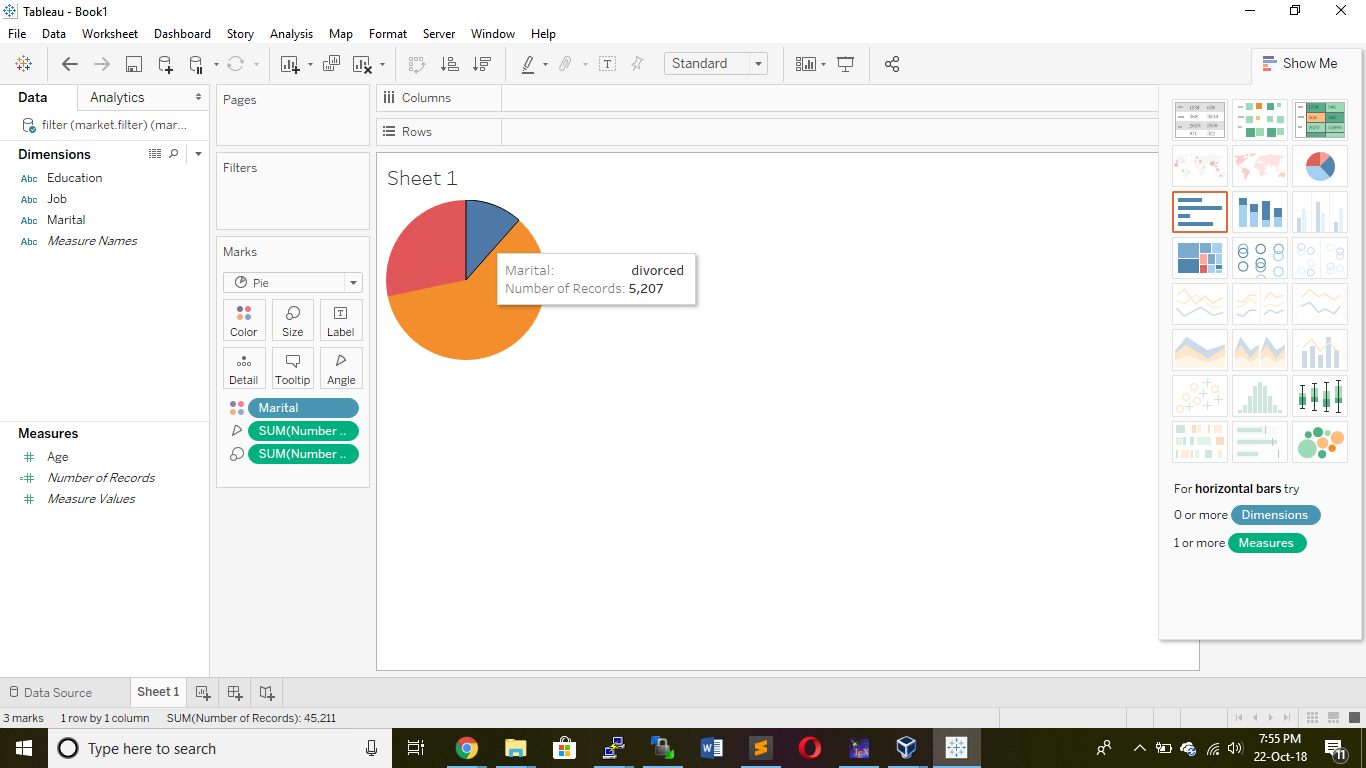
\includegraphics[width=\linewidth]{sc4.png}
	\caption{Pie chart of divorced vs count}
\end{figure}
\\
\\
Bank - Job Graph looks like-
\begin{figure}[h!]
	\centering
	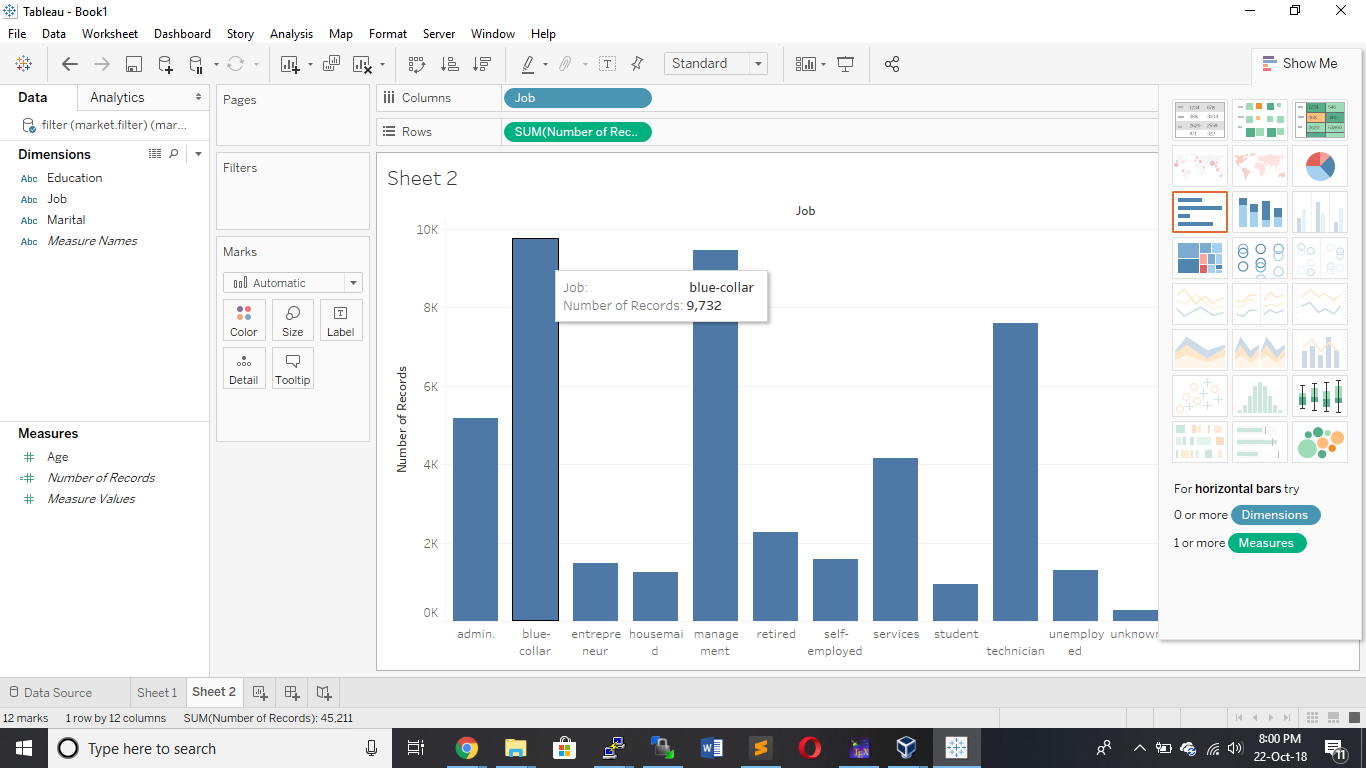
\includegraphics[width=\linewidth]{sc6.png}
	\caption{Job vs Count}
\end{figure}
\\
\\
Job profile for Teachnician-
\begin{figure}[h!]
	\centering
	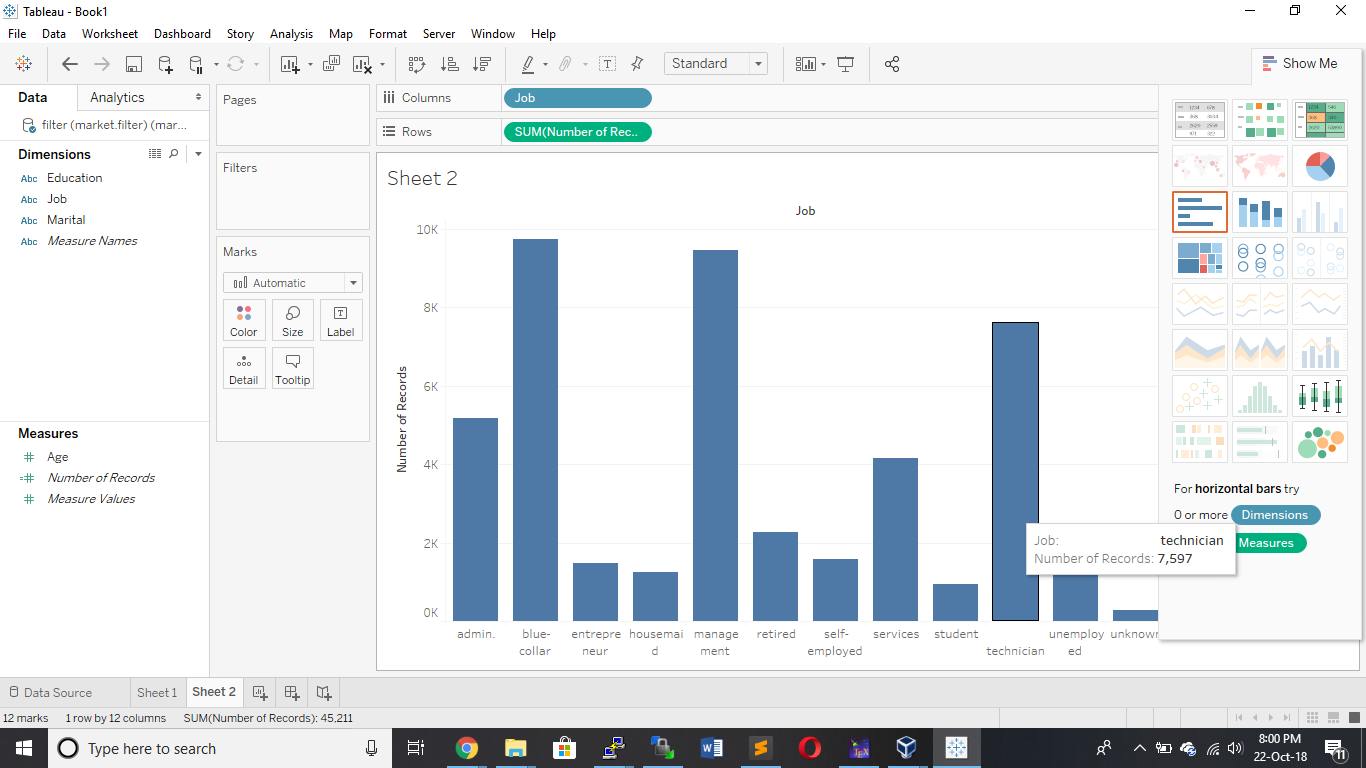
\includegraphics[width=\linewidth]{sc7.png}
	\caption{Job record for Teachnician }
\end{figure}
\\
\\
Bank - Education Graph looks like-
\begin{figure}[h!]
	\centering
	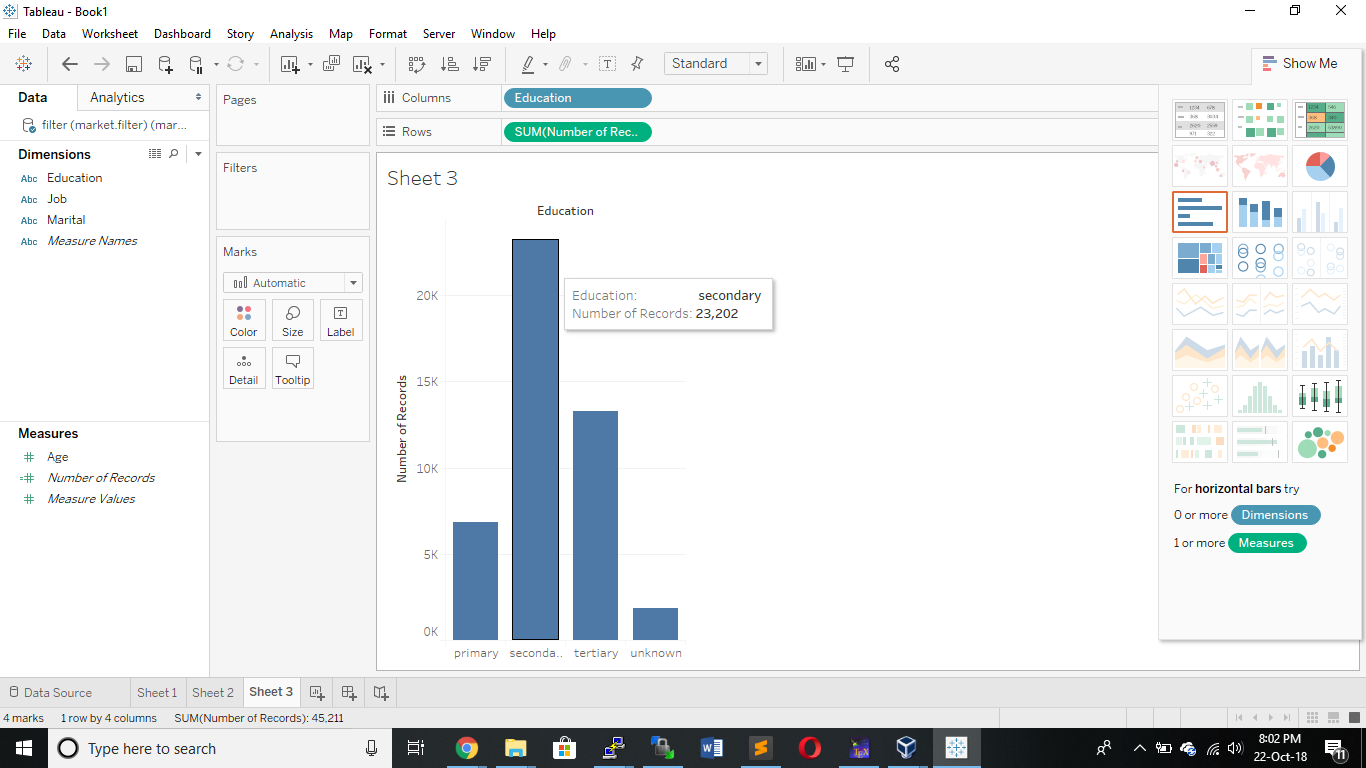
\includegraphics[width=\linewidth]{sc8.png}
	\caption{Education vs record}
\end{figure}
\\
\\
%
Bank - Age Graph look like- 
\begin{figure}[h!]
	\centering
	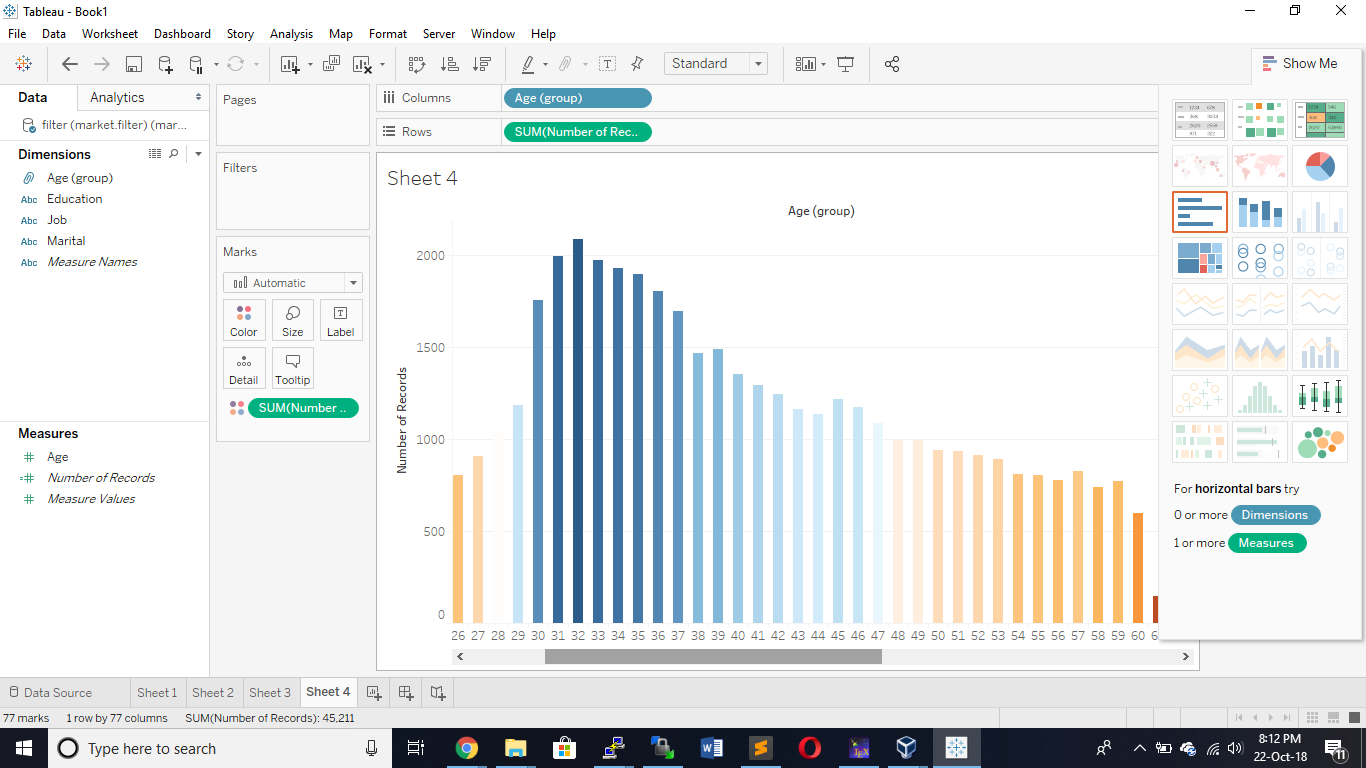
\includegraphics[width=\linewidth]{sc9.png}
	\caption{Age vs record}
\end{figure}
%
\\
\\



\section{Testing}
Big data is a collection of large datasets that cannot be processed using traditional computing techniques. Testing of these datasets involves various tools, techniques and frameworks to process. Big data relates to data creation, storage, retrieval and analysis that is remarkable in terms of volume, variety, and velocity.
\\
\\
Testing Big Data application is more a verification of its data processing rather than testing the individual features of the software product. When it comes to Big data testing, performance and functional testing are the key.
\\
\\
In Big data testing QA engineers verify the successful processing of terabytes of data using commodity cluster and other supportive components. It demands a high level of testing skills as the processing is very fast. Processing may be of three types
\begin{itemize}
	\item Batch
	\item Real Time
	\item Interactive
\end{itemize}
\\
\\
Along with this, data quality is also an important factor in big data testing. Before testing the application, it is necessary to check the quality of data and should be considered as a part of database testing. It involves checking various characteristics like conformity, accuracy, duplication, consistency, validity, data completeness, etc.

\subsection{Testing Steps in verifying Big Data Applications}
\\
The following figure gives a high level overview of phases in Testing Big Data Applications
\begin{figure}[h!]
	\centering
	\includegraphics[width=\linewidth]{TestingBigData.png}
	\caption{Testing BigData}
\end{figure}
\\
Big Data Testing can be broadly divided into three steps
\\
\textbf{Step 1: Data Staging Validation}
\\
The first step of big data testing, also referred as pre-Hadoop stage involves process validation.
\begin{itemize}
	\item Data from various source like RDBMS, weblogs, social media, etc. should be validated to make sure that correct data is pulled into system.
	\item Comparing source data with the data pushed into the Hadoop system to make sure they match.
	\item Verify the right data is extracted and loaded into the correct HDFS location.
\end{itemize}
\\
Tools like Talend, Datameer, can be used for data staging validation
\\
\textbf{Step 2: "MapReduce" Validation}
\\
The second step is a validation of "MapReduce". In this stage, the tester verifies the business logic validation on every node and then validating them after running against multiple nodes, ensuring that the
	\begin{itemize}
		\item Map Reduce process works correctly
		\item Data aggregation or segregation rules are implemented on the data
		\item Key value pairs are generated
		\item Validating the data after Map Reduce process
	\end{itemize}
\\
\textbf{Step 3: Output Validation Phase}
\\
The final or third stage of Big Data testing is the output validation process. The output data files are generated and ready to be moved to an EDW (Enterprise Data Warehouse) or any other system based on the requirement.
\\
Activities in third stage includes
\begin{itemize}
	\item To check the transformation rules are correctly applied
	\item To check the data integrity and successful data load into the target system
	\item To check that there is no data corruption by comparing the target data with the HDFS file system data
\end{itemize}
\\
\subsection{Architecture Testing}
\\
Hadoop processes very large volumes of data and is highly resource intensive. Hence, architectural testing is crucial to ensure success of your Big Data project. Poorly or improper designed system may lead to performance degradation, and the system could fail to meet the requirement. Atleast, Performance and Failover test services should be done in a Hadoop environment.

Performance testing includes testing of job completion time, memory utilization, data throughput and similar system metrics. While the motive of Failover test service is to verify that data processing occurs seamlessly in case of failure of data nodes

\subsection{Performance Testing}
Performance Testing for Big Data includes two main action
\begin{itemize}
	\item Data ingestion and Throughout: In this stage, the tester verifies how the fast system can consume data from various data source. Testing involves identifying different message that the queue can process in a given time frame. It also includes how quickly data can be inserted into underlying data store for example insertion rate into a Mongo and Cassandra database.
	\item Data Processing: It involves verifying the speed with which the queries or map reduce jobs are executed. It also includes testing the data processing in isolation when the underlying data store is populated within the data sets. For example running Map Reduce jobs on the underlying HDFS
	\item Sub-Component Performance: These systems are made up of multiple components, and it is essential to test each of these components in isolation. For example, how quickly message is indexed and consumed, mapreduce jobs, query performance, search, etc.
\end{itemize}


\subsection{Test Environment Needs}
Test Environment needs depend on the type of application you are testing. For Big data testing, test environment should encompass
\begin{itemize}
	\item It should have enough space for storage and process large amount of data
	\item It should have cluster with distributed nodes and data
	\item It should have minimum CPU and memory utilization to keep performance high
\end{itemize}
	
\chapter{Conclusion and Future Scope}\hrule
\label{Chapter:5}
% =====================================================================================================
\section{Conclusion}
This projectt has implemented Data Visualization, Cross-Tabulation,Data Clustering,  Analysis Data Correlation and Cross Validation in order to verify that it is possible to predict Term Deposit successes with Bank Marketing client data.

Data Clustering demonstrated the similarity of the Bank Marketing clients, and the non-presence of outlier data points. Correlation Analysis demonstrated that the dataset variables that have the most correlation with Term Deposit subscription are “Housing” and “Loan”. The accuracy of the predictions are verified with a Probability Value of 0.6681 and a 95 percent confidence interval of -0.03721581 to 0.0238623.
\section{Future Scope}
The Project has been keeping in mind of future feature additions.\\
Due to Digitalization and other factors have made things accessible while simultaneously making it difficult to keep data structured and well-managed.\\
The Project has main moto to increase revenue of Bank and make them increases marketing. I hope,this Project will achieve its aim of development and will generate a great revenue for Bank Institution.
\chapter{Refrences}\hrule
\label{Chapter:6}
% =====================================================================================================
\begin{enumerate}
	\item https://hadoop.apache.org/ [accesed on 13/06/2018]
	\item http://www.rpubs.com/johnakwei/330635 [accesed on  14/06/2018]
	\item https://www.cloudera.com/ [accesed on 15/06/2018]
	\item https://www.putty.org/ [accesed on 15/06/2018]
	\item https://winscp.net/eng/download.php [accesed on 15/06/2018]
	\item https://www.tutorialspoint.com/hadoop/ [accesed on 16/06/2018]
	\item https://www.tableau.com/ [accesed on 28/06/2018]
	\item https://www.guru99.com/big-data-testing-functional-performance.html [accesed on 08/07/2018]
	\item https://www.edureka.co/blog/hadoop-tutorial/ [accesed on 09/07/2018]
	\item https://stackoverflow.com/questions/tagged/hadoop [accesed on 10/07/2018]
	\item https://www.draw.io/ [accesed on 05/08/2018]
\end{enumerate}